\documentclass[conference]{IEEEtran}
\usepackage{amsmath,amssymb}
\usepackage{booktabs}
\usepackage{array}
\usepackage{xcolor}
\usepackage{url}
\usepackage{graphicx}
\usepackage{dblfloatfix}
\usepackage{capt-of}
\usepackage{titlesec}

\newcommand{\um}{\ensuremath{\mu\mathrm{m}^2}}
\renewcommand{\thesection}{\arabic{section}}
\renewcommand{\thesubsection}{\thesection.\arabic{subsection}}
\renewcommand{\thesubsubsection}{\thesubsection.\arabic{subsubsection}}
\renewcommand{\thesectiondis}{\thesection}
\renewcommand{\thesubsectiondis}{\thesubsection}
\renewcommand{\thesubsubsectiondis}{\thesubsubsection}
\titleformat{\section}
  {\normalfont\large\bfseries}{\thesection}{1em}{}
\titleformat{\subsection}
  {\normalfont\large\bfseries}{\thesubsection}{0.8em}{}
\titleformat{\subsubsection}
  {\normalfont\normalsize\bfseries}{\thesubsubsection}{0.8em}{}
\titlespacing*{\section}{0pt}{1.6ex plus 0.6ex minus 0.2ex}{0.8ex}
\titlespacing*{\subsection}{0pt}{1.2ex plus 0.4ex minus 0.2ex}{0.6ex}
\titlespacing*{\subsubsection}{0pt}{1.0ex plus 0.3ex minus 0.2ex}{0.4ex}

\title{OADM: A Runtime-Configurable Shared Approximate\\
FP32 Divider--Multiplier}
\author{\IEEEauthorblockN{Pingchuan Dong}
}

\begin{document}
\maketitle

\begin{abstract}
Approximate floating-point division and multiplication are often implemented
as separate datapaths despite their related mantissa arithmetic. OADM is a
runtime-configurable approximate FP32 divider--multiplier derived from
tangent-plane approximations. Its divide and multiply planes share mantissa
partitioning, midpoint selection, plane evaluation, and the floating-point
front/back-end; division alone applies a reciprocal-square scale. A runtime control selects L0--L3 in one hardware instance, while fixed-level
wrappers tie this control during synthesis so that each level's standalone
PPA can be measured. Bit-exact centered-residual
implementations reduce the cost of the common plane. RTL equivalence tests and
a common TSMC 65-nm Design Compiler/PrimeTime flow quantify the level tradeoff,
the area retained through sharing, the gap to an unshared exact DIV+MUL
reference, and the DIV-only comparison with a reproduced PACE divider.
\end{abstract}

\begin{IEEEkeywords}
approximate computing, floating-point arithmetic, divider, multiplier,
tangent-plane approximation, configurable arithmetic, ASIC
\end{IEEEkeywords}

\section{Introduction}
Floating-point (FP) division remains expensive in numerical, signal-processing,
and learning workloads, even though its sign and exponent operations are
simple; the normalized-mantissa quotient is the costly part. Multiplication and
division are also commonly needed by the same processing element. In
error-tolerant workloads, approximate arithmetic can exchange bounded numerical
error for lower area, delay, and energy. The design opportunity is therefore
broader than a low-cost divider alone: a practical unit should expose an
application-selected accuracy--cost tradeoff while avoiding duplicated mantissa
arithmetic when both operations are present.

Prior approximate dividers show that this goal is nontrivial. Approximate
digit-recurrence designs simplify a non-restoring or dynamic divider
core~\cite{chen2015nonrestoring,hashemi2016dynamic}. Logarithmic and
mantissa-subtraction designs replace division with a simpler domain transform
or subtraction, as in CADE, LEAD, and FaNZeD
\cite{imani2019cade,ratnaparkhi2022lead,saadat2019fanzed}. Reciprocal-based
designs refine or interpolate $1/y$ before combining it with the dividend;
SAADI-EC, ILAFD, QIAD, and PACE illustrate different choices of iteration,
interpolation, and error compensation
\cite{melchert2019saadi,oelund2023ilafd,liu2023qiad,wen2025pace}. A separate
line of work fits local planes directly to the division surface
\cite{wu2015curve,wu2024plsad}. These approaches make different tradeoffs
among accuracy, latency, and circuit cost. Prior combined multiplier--divider
work such as SIMDive also demonstrates the value of one configurable operation
block, but it is a Mitchell-based integer/SIMD architecture targeted to FPGA
fabrics~\cite{ebrahimi2020simdive}.

OADM is derived from the OAM multiplier plane~\cite{chen2020oam} and the OAD
divider formulation~\cite{oad2023}. Through algebraic transformation, we discovered a direct connection between the multiplier and divider planes, so the approximate multiplier and divider share mantissa partitioning, residual
formation, midpoint selection, and plane evaluation. In hardware terms, this indicates significant area overlap, therefore we decided to implement an approximate fp32 divider-multiplier that leverages this sharing.
On the top level, an input selects operation from division and multiplication, and the level input
selects L0--L3 at runtime according to the need for precision. OADM is consequently a shared arithmetic core, rather than two approximate
units selected by an output mux. The derivation section explains the OAD/OAM
connection needed to establish that claim, then  the circuit implementation offers a few tweaks in the hardware implementation to optimize the performance while realizing the core approximation algorithm.

The contributions of this work are as follows:
\begin{itemize}
  \item We derived the algebraic relation between the OAD divider plane
  and the OAM multiplier plane, showing that both operations can be expressed
  using the same midpoint-dependent primitive terms with an operation-dependent
  sign. We translate this relation into a shared FP32 divider--multiplier
  datapath whose modes share partitioning, residual formation, midpoint
  selection, and tangent-plane evaluation; division additionally applies its
  reciprocal-square scale.

  \item We provide runtime selection of both operation and approximation level
  (L0--L3). The same RTL supports an application-selected accuracy--cost point,
  while fixed-level elaborations expose the PPA of each selected level without
  charging unused runtime logic to that characterization.

  \item We develop bit-exact centered-residual implementations of the shared
  plane and identify complementary L3 Pareto points: centered residual for
  area/power and a subtractor-free residual form for delay.

  \item We evaluate the shared block and its divider mode under explicit,
  separate comparison boundaries: an unshared DesignWare DIV+MUL reference for
  the full operator and reproduced PACE RTL for DIV-only. The common TSMC65
  DC/PT flow and mode-tied ablation quantify both PPA and the area retained by
  structural sharing.
\end{itemize}
\section{Related Work}
\subsection{Approximate FP Division}
Approximate dividers can be grouped by the arithmetic they simplify.
Truncation and approximate digit-recurrence designs reduce work in a restoring,
non-restoring, or subtractor-array-style core. Chen \emph{et al.} simplify a
non-restoring divider, Hashemi \emph{et al.} introduce a dynamic approximate
divider, and TruncApp truncates divider computation
\cite{chen2015nonrestoring,hashemi2016dynamic,vahdat2017truncapp}. They retain
a familiar quotient-generation structure, although an array implementation can
still have substantial logic depth or require a reduced exact core. Logarithmic
designs use a leading-one detector and an approximation to $\log_2(1+f)$ so
that division becomes subtraction in the log domain. LEAD and FaNZeD are
representative examples~\cite{ratnaparkhi2022lead,saadat2019fanzed}. CADE
similarly replaces FP mantissa division with subtraction and uses a runtime
tuning table for error correction~\cite{imani2019cade}.

Reciprocal-based dividers approximate $1/y$ before combining it with the
dividend. SAADI-EC incrementally refines a reciprocal through Taylor-series
terms, while ILAFD combines an approximate reciprocal with an iterative
logarithmic multiplier~\cite{melchert2019saadi,oelund2023ilafd}. QIAD uses
quadratic interpolation, whereas PACE uses a piecewise reciprocal formulation
formed from shifts, additions, and level-wise error compensation
\cite{liu2023qiad,wen2025pace}. The approach can be accurate, but a
conventional reciprocal datapath often needs one or more multipliers.
Surface-fitting designs approximate the mantissa surface $x/y$ directly with
local planes. Wu \emph{et al.} introduced an earlier curve-fitting divider,
and PLSAD combines piecewise linear fitting with coefficient realization and
an approximate lower-part adder~\cite{wu2015curve,wu2024plsad}. The categories
overlap in individual designs, but they expose an important limitation for this
work: a DIV-only approximation does not by itself yield a low-cost multiplier
that shares its arithmetic.

OADM builds on a different observation. The locally optimal OAD divider plane
and OAM multiplier plane have a common midpoint-partition structure and
related level-wise corrections. Unlike the DIV-only architectures above, it
makes that algebraic relation an architectural objective: one
runtime-configurable datapath implements either operation without duplicating
partition, residual, and plane logic. SIMDive is the closest conceptual prior
work in offering a unified configurable multiplier/divider, but it shares
Mitchell log-domain arithmetic for FPGA SIMD lanes rather than an FP32
tangent-plane core~\cite{ebrahimi2020simdive}. The paper evaluates integer
8--32-bit lanes on FPGA; its native results are consequently not a like-for-like
ASIC FP32 baseline. Section~\ref{sec:simdive-context} reports only a clearly
labeled local integer-core FP32-wrapper context.

\section{Derivation and Runtime Configurability}
Comparing to integer computing, FP arithmetic is more complex and so energy consuming. According to IEEE 754 standard in \cite{Ieee}, an FP number $F_{x} $ consists of
sign, mantissa and exponent as follows:
\[F_{x}=sign_{x}\times x\times 2^{E_{x}},\;\forall x\in [1, 2)\]
where $sign_{x}, x, E_{x}$ refer to the sign, mantissa and exponent of $F_{x}$ respectively. Thus for two FP numbers $F_{x}$ and $F_{y}$, the division is:
$${F_{x}\over F_{y}}=sign_{x}sign_{y}\times {x\over y}\times 2^{E_{x}-E_{y}}.$$
In a general processor, for an FP division, the sign bits is computed by an XOR operation and the exponent bits are computed by a subtractor. The division ${x\over y}$ of two mantissas is much more energy consuming and costlier than the computations of signs and exponents. The motivation of this work is to propose an energy efficient divider for ${x\over y}$ between mantissas.

\subsection{Preliminaries: OAM}
OAM approximates the mantissa product in FP multiplication after the same
front-end decomposition. The exact mantissa product is $h(x,y)=xy$. OAM divides
the mantissa domain into local
rectangular regions and replaces $h(x,y)$ in each region by a tangent plane.
For a generic cell $[x_1,x_2]\times[y_1,y_2]$, let the tangent point be
$(k_x,k_y)$. The first-order expansion of $xy$ at this point gives
\begin{equation}
\begin{aligned}
\widehat{m}
&= k_xk_y+k_y(x-k_x)+k_x(y-k_y) \\
&= -k_xk_y+k_yx+k_xy .
\end{aligned}
\label{eq:oam_plane_prelim}
\end{equation}
The OAM formulation chooses the tangent point by minimizing the integral error
over the cell. With
\begin{equation}
E_M(k_x,k_y)=\int_{x_1}^{x_2}\int_{y_1}^{y_2}
\left[xy-(-k_xk_y+k_yx+k_xy)\right]\,dy\,dx,
\end{equation}
the stationarity conditions yield
\begin{equation}
k_x={x_1+x_2\over2},\qquad k_y={y_1+y_2\over2}.
\label{eq:oam_midpoint_prelim}
\end{equation}
Thus the selected tangent point is simply the midpoint of the local mantissa
cell. At level $n$, OAM partitions each mantissa axis into $2^n$ intervals. If
$i_x^n$ and $i_y^n$ are the selected interval indices, the corresponding
midpoints are
\begin{equation}
k_x^n=1+\left(i_x^n+{1\over2}\right)2^{-n},\qquad
k_y^n=1+\left(i_y^n+{1\over2}\right)2^{-n}.
\end{equation}
The level therefore controls how fine the local plane is: L0 uses one plane
over the whole normalized domain, while L1--L3 progressively refine the
partition. OADM starts from this OAM structure and asks whether the divider's
mantissa quotient can be expressed with the same midpoint partition and the
same elementary plane terms.

\subsection{Divider Tangent-Plane Equation Derivation}
\subsubsection{Direct Derivation}
For any local cell $[x_1,x_2]\times[y_1,y_2]\subset[1,2)\times[1,2)$, OAD first
approximates the divider surface $z=x/y$ directly. The tangent plane at
$(x_0,y_0,z_0=x_0/y_0)$ is
\begin{equation}
z={x_0\over y_0}+{1\over y_0}(x-x_0)-{x_0\over y_0^2}(y-y_0)
={1\over y_0}x-{x_0\over y_0^2}y+{x_0\over y_0}.
\end{equation}
The tangent point is chosen by minimizing the integral error over the cell:
\begin{equation}
\begin{aligned}
E_D(x_0,y_0)
&=\int_{x_1}^{x_2}\int_{y_1}^{y_2}
\left[{x\over y}-\left({x_0\over y_0}+{1\over y_0}x
-{x_0\over y_0^2}y\right)\right]\,dy\,dx .
\end{aligned}
\end{equation}
Let $A=x_2-x_1$, $B=y_2-y_1$, $S_x=(x_2^2-x_1^2)/2$, and
$S_y=(y_2^2-y_1^2)/2$. The stationarity conditions are
\begin{equation}
{\partial E_D\over\partial x_0}=-{AB\over y_0}+{A S_y\over y_0^2}=0,
\end{equation}
and
\begin{equation}
{\partial E_D\over\partial y_0}=
{x_0AB\over y_0^2}+{S_xB\over y_0^2}-{2x_0A S_y\over y_0^3}=0.
\end{equation}
They give
\begin{equation}
y_0={S_y\over B}={y_1+y_2\over2},\qquad
x_0={S_x\over A}={x_1+x_2\over2}.
\end{equation}
Thus the locally optimized tangent point is the cell midpoint. With
$k_x=(x_1+x_2)/2$ and $k_y=(y_1+y_2)/2$, the divider approximation is
\begin{equation}
\widehat{d}={k_x\over k_y}+{1\over k_y}(x-k_x)-{k_x\over k_y^2}(y-k_y)
={k_xk_y+k_yx-k_xy\over k_y^2}.
\label{eq:direct_divider_plane}
\end{equation}

\subsubsection{OAM-Based Equivalent Derivation}
The same divider plane can also be obtained from a shorter construction that
uses the OAM product plane. On $[y_1,y_2]$, approximate $1/y$ by the tangent
line at $p$,
\begin{equation}
g(y)=-{y\over p^2}+{2\over p}.
\end{equation}
Choosing $p$ to minimize the integral error gives
\begin{equation}
0=E'_R(p)=(y_1^2-y_2^2)p^{-3}+2(y_2-y_1)p^{-2},
\end{equation}
and therefore $p=(y_1+y_2)/2=k_y$. Combining this reciprocal tangent with the
OAM product approximation in \eqref{eq:oam_plane_prelim} gives
\begin{equation}
\begin{aligned}
{x\over y}
&=x\cdot{1\over y}
\approx -{1\over k_y^2}xy+{2\over k_y}x \\
&\approx -{1\over k_y^2}(-k_xk_y+k_yx+k_xy)+{2\over k_y}x \\
&={1\over k_y^2}(k_xk_y+k_yx-k_xy).
\end{aligned}
\label{eq:oam_based_divider_plane}
\end{equation}
Equations~\eqref{eq:direct_divider_plane} and
\eqref{eq:oam_based_divider_plane} produce the same local divider formula:
the direct OAD optimization reaches the same plane that emerges from the OAM
multiplier plane plus a reciprocal approximation.

\subsection{Architecture for Multi-Level Approximate Divider}
The two derivations above give a level-independent local form for division.
For the level-$n$ rectangular cell containing $(x,y)$, let $k_x^n$ and
$k_y^n$ denote the midpoint coordinates. OAD approximates the mantissa quotient
as
\begin{equation}
 \widehat{d}_n=\frac{w_n}{(k_y^n)^2},\qquad
 w_n=k_x^nk_y^n+k_y^nx-k_x^ny. \label{eq:divplane}
\end{equation}
For the same cell and midpoint, OAM approximates the mantissa product as
\begin{equation}
 \widehat{m}_n=z_M^n=-k_x^nk_y^n+k_y^nx+k_x^ny. \label{eq:mulplane}
\end{equation}
Thus the divider numerator and multiplier plane use the same partition,
midpoint coordinates, and primitive terms, while division changes the sign of
the $k_x^ny$ contribution and scales the numerator by the reciprocal-square
constant $1/(k_y^n)^2$.

Figure~\ref{fig:runtime-arch} summarizes how this selected-level formulation
extends to the complete FP32 divider--multiplier. The operation modes share the
partition midpoints and the three primitive plane terms, while division alone
selects the reciprocal-square scale and multiplication bypasses it.

\begin{figure*}[!t]
\centering
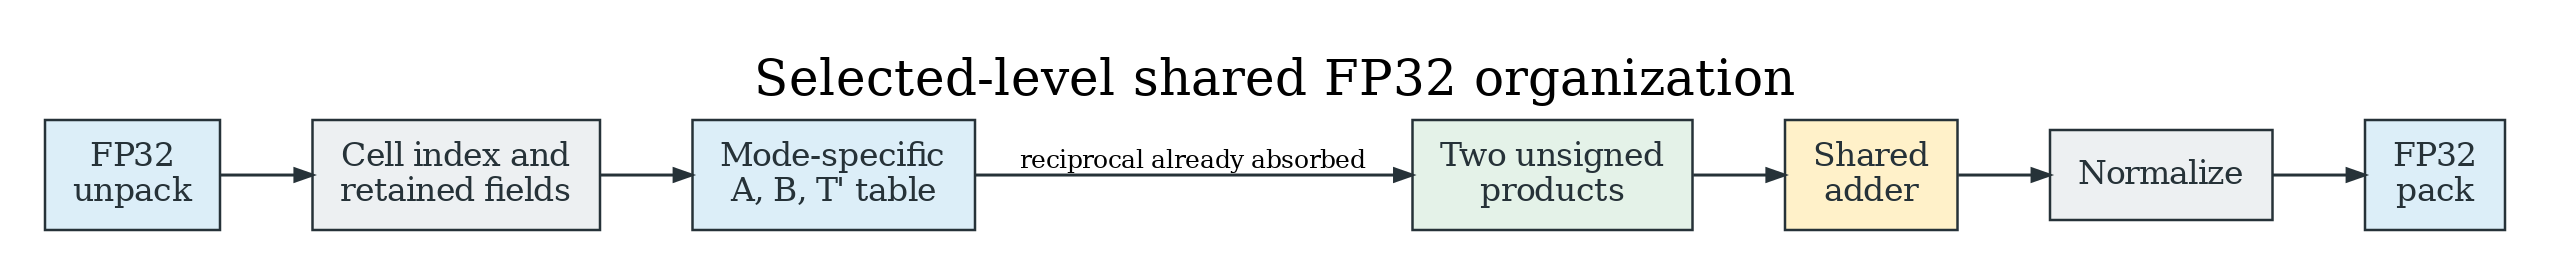
\includegraphics[width=0.96\textwidth]{pictures/structure.png}
\caption{Shared selected-level organization of the proposed OADM FP32
divider--multiplier. DIV and MUL use a common local-plane datapath, with the
reciprocal-square scale enabled only for division.}
\label{fig:runtime-arch}
\end{figure*}

The level input selects one local plane directly rather than enabling a chain
of corrections from L0 to the requested level. This distinction preserves the
algebraic sharing between DIV and MUL without requiring the inter-level
accumulation of an incremental $\Delta z_i$/$\Delta w_i$ architecture.

The initial FP32 mantissa domain is $[1,2)\times[1,2)$. Level~0 uses this
whole domain as one cell. At level~1, each axis is split at $1.5$, producing
four rectangular subregions. In general, level~$n$ partitions each axis into
$2^n$ equal intervals:
\begin{equation}
 [x_{p-1}^n,x_p^n)\times[y_{q-1}^n,y_q^n),\qquad
 x_p^n=1+{p\over2^n},\quad y_q^n=1+{q\over2^n}.
\end{equation}
Figure~\ref{fig:multilevel-partition} visualizes this recursive subdivision for
L0--L2; L3 continues the same bisection once more along each axis.

The midpoint of the selected cell is therefore
\begin{equation}
 k_x^n=1+{2p(n)-1\over2^{n+1}},\qquad
 k_y^n=1+{2q(n)-1\over2^{n+1}},
\end{equation}
where $p(n)$ and $q(n)$ are determined by the leading mantissa bits of $x$ and
$y$. Equivalently, starting from $k_x^0=k_y^0=3/2$, each deeper level updates
the midpoint by one signed binary step:
\begin{equation}
 k_x^n=k_x^{n-1}+\sigma_x(n)2^{-(n+1)},\qquad
 k_y^n=k_y^{n-1}+\sigma_y(n)2^{-(n+1)}, \label{eq:midpoint_update}
\end{equation}
where $\sigma_x(n),\sigma_y(n)\in\{-1,+1\}$ are selected by the $n$th
fractional bits.

Figure~\ref{fig:selected-partition-point} shows that the same operand pair
$(x,y)$ lies in one cell at each partition level. As the level increases, the
grid becomes finer; the leading mantissa bits identify the finer cell that
contains $(x,y)$, and the center of that cell defines the level-dependent
midpoint $(k_x^n,k_y^n)$ used to evaluate the selected tangent plane.

\begin{figure*}[!b]
\centering
\begin{minipage}[t]{0.55\textwidth}
  \centering
  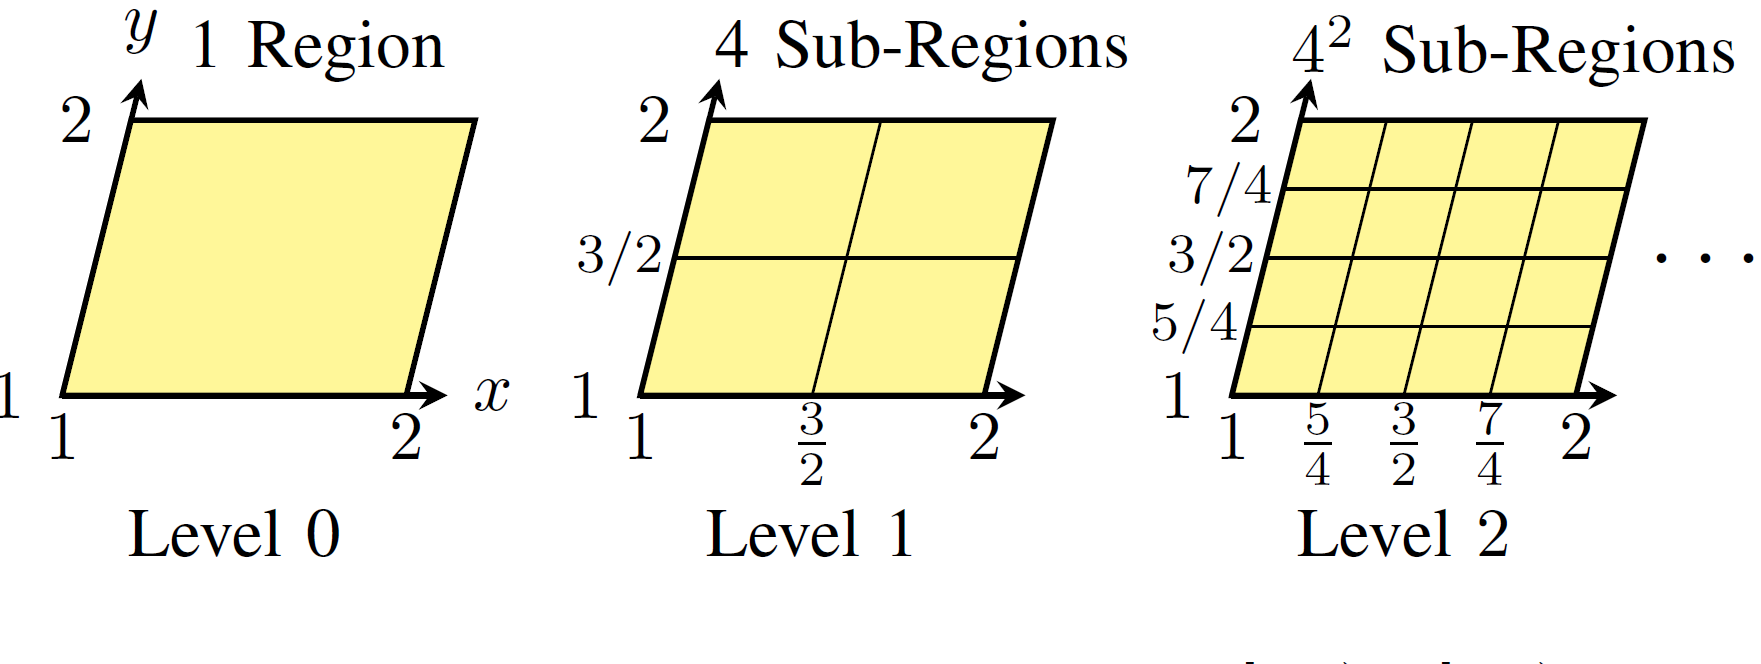
\includegraphics[width=\linewidth,trim=0 19pt 0 0,clip]
    {pictures/Figure 2.png}
  \captionof{figure}{Multi-level partition of the normalized mantissa domain.
  Each level bisects every interval along both axes.}
  \label{fig:multilevel-partition}
\end{minipage}
\hfill
\begin{minipage}[t]{0.38\textwidth}
  \centering
  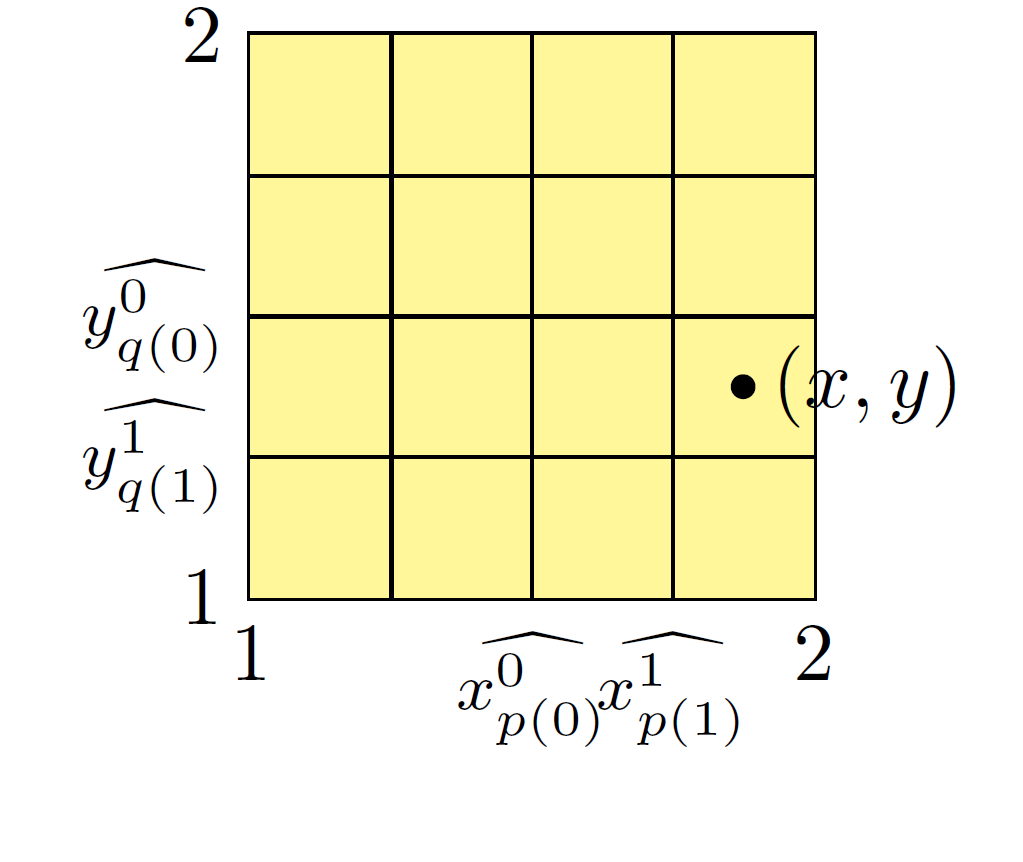
\includegraphics[width=0.86\linewidth,trim=0 20pt 0 0,clip]
    {pictures/Figure 3.png}
  \captionof{figure}{Selection of the local cell and midpoint coordinates for
  a mantissa pair $(x,y)$ in nested partitions.}
  \label{fig:selected-partition-point}
\end{minipage}
\end{figure*}

The remaining divider-specific factor is the reciprocal-square scale. Since
$k_y^n$ is fixed once the level and $y$-interval are known, the scale can be
precomputed and selected from a small table. For the L0--L3 levels used in this
work, the ideal constants are
\begin{align}
\text{L0:}\quad & {1\over(3/2)^2}, \nonumber\\
\text{L1:}\quad &
\begin{cases}
{1\over(5/4)^2}, & y[1]=0,\\
{1\over(7/4)^2}, & y[1]=1,
\end{cases} \nonumber\\
\text{L2:}\quad &
\begin{cases}
{1\over(9/8)^2},  & y[1:2]=00,\\
{1\over(11/8)^2}, & y[1:2]=01,\\
{1\over(13/8)^2}, & y[1:2]=10,\\
{1\over(15/8)^2}, & y[1:2]=11,
\end{cases} \nonumber\\
\text{L3:}\quad &
\begin{cases}
{1\over(17/16)^2}, & y[1:3]=000,\\
{1\over(19/16)^2}, & y[1:3]=001,\\
{1\over(21/16)^2}, & y[1:3]=010,\\
{1\over(23/16)^2}, & y[1:3]=011,\\
{1\over(25/16)^2}, & y[1:3]=100,\\
{1\over(27/16)^2}, & y[1:3]=101,\\
{1\over(29/16)^2}, & y[1:3]=110,\\
{1\over(31/16)^2}, & y[1:3]=111.
\end{cases}
\label{eq:recip_table}
\end{align}
The RTL uses Q0.7 quantized versions of these constants, selected jointly by
the runtime level and the leading fraction bits of $y$.

\section{Circuit Implementation}
The FP32 front end in Figure~\ref{fig:runtime-arch}
extracts signs, exponents, and normalized mantissas once, after which partition
and centered-residual logic feed a single tangent-plane core. The level input
selects the L0--L3 partition granularity and corresponding local plane. The operation input applies the
reciprocal-square scale for division or bypasses it for multiplication. Both
modes then use the same normalizer and packer, unlike separate DIV and MUL
cores joined only by an output mux.

Centered residuals represent each mantissa around its local midpoint, reducing
residual width without changing the selected-level bit result. For the fixed
L3 implementation, the subtractor-free variant replaces
offset-binary-to-two's-complement conversion with an MSB inversion. It provides
the delay Pareto point, while centered-residual L3 provides the area/power
point. The runtime area/power point uses the same subtractor-free residual
recoding, but keeps the level selector live. All variants use the same FP32
interface and Q0.7 divider coefficients; subnormals are flushed rather than
gradually normalized.

The fixed L2 DIV-only implementation additionally propagates its level
constants before synthesis. Its midpoint numerators are
$M_x=9+2i_x$ and $M_y=9+2i_y$ in Q3, and the constant product is formed as
$M_xM_y=81+18(i_x+i_y)+4i_xi_y$. Bounds over all L2 cells remove unreachable
normalizer branches. A separate area/power variant additionally exploits the
fact that the unscaled centered plane is positive and strictly below four,
retaining only 25 active Q23 bits before reciprocal scaling. Both variants are
exact specializations of the same Q0.7 centered-residual result, not additional
arithmetic approximations; the delay-balanced variant is selected for L2.

\subsection{Runtime Centered-Residual Plane}
The runtime implementation used in Table~\ref{tab:full} keeps the level input
live while still evaluating the selected tangent plane in centered-residual
form. Let $m_x$ and $m_y$ denote the 24-bit normalized mantissa integers, so
that the hidden bit is one and the binary point is after bit 23. For level
$n\in\{0,1,2,3\}$, the RTL forms local interval indices
\begin{equation}
 i_x^n =
 \begin{cases}
  0, & n=0,\\
  \lfloor(m_x-2^{23})/2^{23-n}\rfloor, & n>0,
 \end{cases}
 \qquad
 i_y^n =
 \begin{cases}
  0, & n=0,\\
  \lfloor(m_y-2^{23})/2^{23-n}\rfloor, & n>0.
 \end{cases}
\end{equation}
Equivalently, these are the leading $n$ fraction bits. The midpoint is
represented as a Q4 integer $K=16k$. Using
\begin{equation}
 B_n\in\{24,20,18,17\},\qquad S_n\in\{0,8,4,2\},
\end{equation}
for levels L0--L3, respectively, the selected midpoint integers are
\begin{equation}
 K_x^n=B_n+S_n i_x^n,\qquad K_y^n=B_n+S_n i_y^n .
\end{equation}
Thus L3 uses $K=17+2i$, corresponding to the midpoint sequence
$17/16,19/16,\ldots,31/16$.

A direct centered implementation would compute
$r_x^n=m_x-K_x^n2^{19}$ and $r_y^n=m_y-K_y^n2^{19}$ with explicit subtractors.
The selected runtime datapath avoids those subtractors. Within each selected
interval, subtracting the midpoint is exactly the same as interpreting the
lower residual field as offset binary and converting it to two's complement.
The hardware therefore inverts the local residual MSB and sign-extends the
remaining bits:
\begin{equation}
\begin{aligned}
 r_x^0 &= \{\,\overline{x_{22}},x_{21:0}\,\},\\
 r_x^1 &= \mathrm{sext}\{\,\overline{x_{21}},x_{20:0}\,\},\\
 r_x^2 &= \mathrm{sext}\{\,\overline{x_{20}},x_{19:0}\,\},\\
 r_x^3 &= \mathrm{sext}\{\,\overline{x_{19}},x_{18:0}\,\},
\end{aligned}
\label{eq:runtime_residual}
\end{equation}
and symmetrically for $r_y^n$. This is a wiring/inversion recoding of
$m-K2^{19}$, not an arithmetic subtractor.

The runtime plane then uses one pair of residual-by-midpoint products and one
shared constant term:
\begin{align}
 C_n &= (K_x^nK_y^n)2^{15},\\
 T_x &= (r_x^nK_y^n) \gg 4,\qquad
 T_y = (r_y^nK_x^n) \gg 4.
\end{align}
For multiplication the shared plane is $C_n+T_x+T_y$; for division it is
$C_n+T_x-T_y$ before the reciprocal-square scale. The same two rounding-error
LUT lookups used by the fixed-level planes are selected by the runtime
indices, and their small correction is subtracted from either mode. Division
then multiplies the shared value by the Q0.7 coefficient selected from the
$K_y^n$ table, while multiplication bypasses that scale. Both modes finally
enter the same normalization and FP32 packing logic.

\section{Evaluation and Discussion}
\subsection{Evaluation Protocol}
All reported PPA uses Design Compiler U-2022.12-SP7 and PrimeTime
U-2022.12-SP5 with the TSMC 65-nm typical CCS library. The designs are
combinational, with no clock port or sequential area. The 10-ns virtual clock
has zero uncertainty, 20-ps input/output delays, an \texttt{INVD0} input
driver, and 0.004 output load. PT reads the synthesized netlist and SDC,
checks timing, and applies static probability 0.5 and toggle rate 0.1 per
10-ns period to all inputs. Every local structural comparison uses the same
explicit flattening and post-map \texttt{optimize\_netlist -area} policy.
All canonical netlists are combinational, single-module standard-cell mappings
without macros or black boxes.

The exact full reference instantiates DesignWare \texttt{DW\_fp\_div} and
\texttt{DW\_fp\_mult} in parallel, followed by a \texttt{divide\_mode} output
mux. Because it contains no cross-operation sharing, it is the appropriate
exact reference for a full OADM DIV+MUL block. PACE remains a DIV-only
comparison and is evaluated only against OADM's fixed-level normalized-finite
FP32 divider wrappers. Both use the same DC/PT flow and the same fixed-seed
set of 10,000 positive normalized FP32 operand pairs for MAE, MRED, and RMSE.
Where available, prior RTL uses the same normal-FP32 wrapper; LEAD is reported
as a combinational unroll verified to match its supplied two-phase RTL.

\subsection{SIMDive-Derived Integer-Core FP32-Wrapper Context}
\label{sec:simdive-context}
SIMDive is an integer, variable-precision FPGA architecture, not a native
IEEE-754 unit~\cite{ebrahimi2020simdive}. To establish a useful boundary for
runtime DIV+MUL hardware, we wrap the authors' supplied single-32-bit integer
core with a local FP32 sign/exponent/unpack/pack shell. The experiment accepts
only normal finite FP32 operands. For division, the 24-bit normalized dividend
mantissa is shifted left by eight bits before entering the integer core, so the
returned quotient has Q8 fractional precision before FP32 repacking. Zero is
flushed and subnormal or non-finite inputs follow a documented non-IEEE
fallback.

Table~\ref{tab:simdive} gives the resulting local data. The authors' core,
the wrapper, and the synthesized netlist are combinational and use the same
explicitly flattened TSMC65 10-ns DC/PT flow as OADM. The author source has a 32-to-31-bit
\texttt{shifter\_out} connection that event-driven simulators truncate
implicitly. For synthesis, a compatibility declaration makes that truncation
explicit while preserving the same deterministic 10,000-vector RTL error
statistics. A 20,000-vector check generated expected outputs with two-state
RTL simulation and reproduced them with the synthesized gate netlist.

\begin{table*}[t]
\caption{SIMDive-derived integer-core FP32-wrapper context. Accuracy uses
10,000 deterministic positive normalized mantissa pairs in $[1,2)$. The PPA
row is one runtime-selectable DIV/MUL wrapper, not a native FP32 SIMDive
implementation.}
\label{tab:simdive}
\centering\small
\begin{tabular}{lrrrrrrrr}
\toprule
Design & DIV MAE & DIV MRED & DIV RMSE & MUL MAE & MUL MRED & MUL RMSE & Area (\um) & PT delay / power \\
\midrule
SIMDive-derived integer-core FP32 wrapper & 0.008370 & 0.007972 & 0.011515 & 0.018707 & 0.008792 & 0.024884 & 2217.24 & 5.09242 ns / 0.068389 mW \\
\bottomrule
\end{tabular}
\end{table*}

The wrapper's delay and vectorless power provide structurally comparable local
PPA context because the SIMDive-derived wrapper and OADM use the same mapping
boundary. Its DIV MRED is
numerically in the range of the middle OADM levels, while its MUL MRED is near
the L1 range. Those accuracy observations are qualitative because the SIMDive
wrapper uses a different deterministic input sequence and a Q8 integer quotient
adapter. Instead, the experiment shows that directly adapting an integer
Mitchell/SIMD core to an FP32 mantissa interface does not reproduce OADM's
tangent-plane sharing formulation.

\subsection{Full DIV+MUL Versus Exact}
Table~\ref{tab:full} reports full-operator PPA. Centered-residual L3 is the
area/power point. Relative to exact selectable DIV+MUL, it reduces area from
20558.16 to 4767.48 \um (76.8\%), power from 1.656330 to 0.229574 mW (86.1\%),
and critical delay from 9.93421 to 4.98826 ns (49.8\%). The subtractor-free
point shortens L3 delay by 3.30\% for 0.12\% more area and 0.38\% more power.
The runtime-selectable centered-residual implementation contains both modes
and all four levels, reaching 5114.88 \um, 5.28936 ns, and 0.232348 mW.

\begin{table*}[t]
\caption{Full selectable DIV+MUL PPA in the 10-ns no-pipeline DC/PT flow}
\label{tab:full}
\centering\small
\begin{tabular}{llrrrl}
\toprule
Design & Variant & Area (\um) & PT delay (ns) & PT power (mW) & Role \\
\midrule
OADM L0 & centered index & 1929.96 & 4.26 & 0.088917 & lowest L0 area/delay \\
OADM L1 & centered residual & 3240.00 & 4.40 & 0.146527 & L1 area/power point \\
OADM L2 & centered residual & 3974.40 & 4.83 & 0.186768 & L2 delay/power point \\
OADM L3 & centered residual & 4767.48 & 4.98826 & 0.229574 & L3 area/power point \\
OADM L3 & subtractor-free residual & 4773.24 & 4.82341 & 0.230443 & L3 delay point \\
OADM runtime L0--L3 & centered residual & 5114.88 & 5.28936 & 0.232348 & runtime area/power point \\
Exact DIV+MUL & unshared DesignWare & 20558.16 & 9.93421 & 1.656330 & exact reference \\
\bottomrule
\end{tabular}
\end{table*}

\subsection{Mode-Tied Sharing Ablation}
To isolate arithmetic sharing, we resynthesized each fixed level in three
forms: DIV-only with \texttt{divide\_mode} tied high, MUL-only with it tied
low, and the selectable DIV+MUL top. All use the same 10-ns no-pipeline DC
flow, allowing synthesis to propagate the operation constant through the
common RTL. Table~\ref{tab:sharing} measures the area avoided by retaining one
plane datapath instead of instantiating two mode-specialized copies. The
selectable unit saves 18.24--22.32\% across L0--L3. This is structural evidence
that the two operations retain common plane arithmetic.

Avoided area grows from 554.04 \um at L0 to 722.88 \um, 902.88 \um, and
1369.80 \um at L1--L3. Deeper levels contain more partition, midpoint, and plane logic
that can be retained once in the selectable unit. The percentage does not rise
monotonically because its denominator also includes level-dependent DIV scaling
and other operation-specific FP32 logic. Absolute saved area is thus the more
informative sharing trend.

All four rows use the centered-residual implementation family, including L0.
This keeps the full, DIV-only, and MUL-only views within each row tied to the
same RTL formulation. The distinct L0 centered-index area/delay point and L3
subtractor-free-residual delay point remain Pareto alternatives in
Table~\ref{tab:full}; neither is mixed into this ablation.

\begin{figure*}[t]
\centering
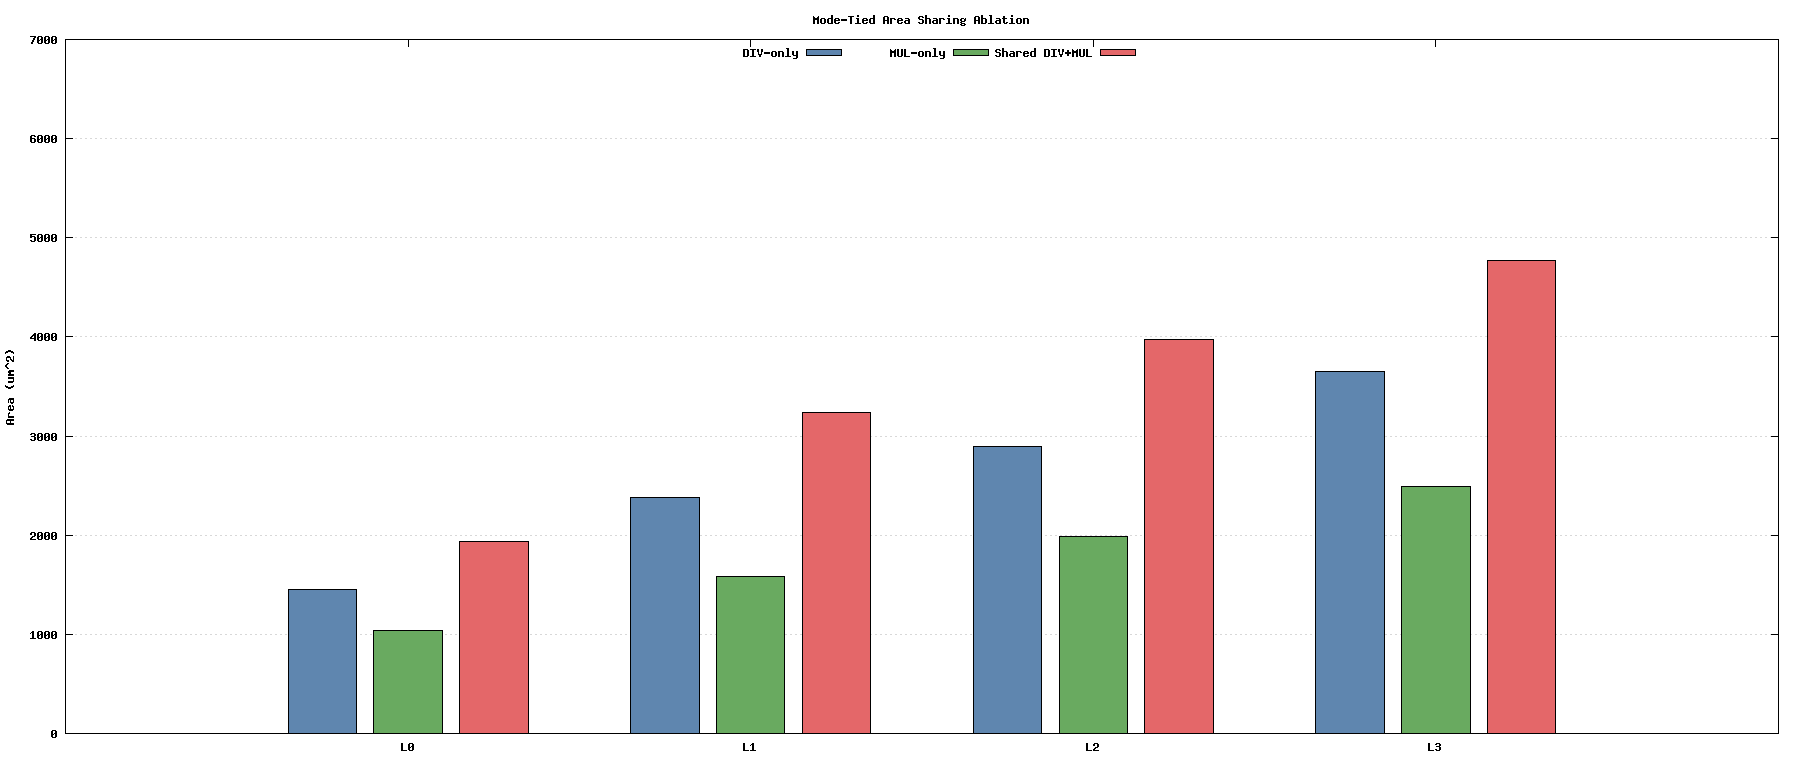
\includegraphics[width=0.94\textwidth]{pictures/sharing_area.png}
\caption{Mode-tied area ablation. The selectable OADM DIV+MUL block retains
one common plane datapath rather than the sum of separate mode-specialized
implementations.}
\label{fig:sharing-area}
\end{figure*}

\begin{table*}[t]
\caption{Mode-tied area sharing ablation, 10-ns no-pipeline DC}
\label{tab:sharing}
\centering\small
\begin{tabular}{lrrrrrr}
\toprule
Level / RTL & DIV-only (\um) & MUL-only (\um) & Separate sum (\um) & Shared DIV+MUL (\um) & Saved (\um) & Saving \\
\midrule
L0 centered residual & 1449.36 & 1036.44 & 2485.80 & 1931.76 & 554.04 & 22.29\% \\
L1 centered residual & 2379.96 & 1582.92 & 3962.88 & 3240.00 & 722.88 & 18.24\% \\
L2 centered residual & 2894.04 & 1983.24 & 4877.28 & 3974.40 & 902.88 & 18.51\% \\
L3 centered residual & 3649.68 & 2487.60 & 6137.28 & 4767.48 & 1369.80 & 22.32\% \\
\bottomrule
\end{tabular}
\end{table*}

\subsection{Strict DIV-Only Comparison with PACE}
PACE is compared only with the OADM DIV-only wrapper. Table~\ref{tab:pace}
uses a fresh Q0.7 RTL accuracy run over 10,000 fixed-seed positive normalized
FP32 operand pairs. The fixed PACE-I/O wrappers match the runtime OADM output
on every vector, so the centered-residual PPA implementations carry the same
reported error. OADM L3 has lower MRED and RMSE than PACE L4, whereas PACE
remains smaller, faster, and lower power. Since PACE has no multiplier mode,
its area is not compared with the full OADM DIV+MUL area in
Table~\ref{tab:full}.

\begin{table*}[t]
\caption{Fair DIV-only OADM/PACE comparison. Accuracy is a fresh
current-Q0.7 RTL run on 10,000 fixed-seed normalized pairs; PPA uses the
same explicitly flattened, area-optimized DC/PT mapping policy. The starred
L2 point applies bit-exact fixed-level midpoint and range specialization.}
\label{tab:pace}
\centering\small
\begin{tabular}{llrrrrr}
\toprule
OADM / PACE & OADM variant & Area (\um) & Delay (ns) & Power (mW) & MRED & RMSE \\
\midrule
L0 / L1 & centered residual & 1285.92 / 668.88 & 3.09370 / 2.04272 & 0.072915 / 0.025703 & 0.042928 / 0.026218 & 0.069134 / 0.045861 \\
L1 / L2 & centered residual & 2145.60 / 1259.64 & 3.60242 / 3.10953 & 0.110179 / 0.053987 & 0.011202 / 0.014993 & 0.019606 / 0.022565 \\
L2 / L3 & centered residual$^\ast$ & 2587.32 / 1853.28 & 3.87981 / 3.42280 & 0.158764 / 0.089690 & 0.008365 / 0.005652 & 0.009490 / 0.009354 \\
L3 / L4 & centered residual & 3373.20 / 2786.04 & 4.07998 / 3.70799 & 0.195428 / 0.132822 & 0.003205 / 0.003834 & 0.004595 / 0.006066 \\
\bottomrule
\end{tabular}
\end{table*}

\subsection{Prior-Work Context and Discussion}
Table~\ref{tab:prior} places locally reproduced DIV-only designs under the
same 10-ns no-pipeline TSMC65 DC/PT flow. PACE L4, FaNZeD, TruncApp, and the
combinational LEAD unroll retain their local wrappers and stated evaluation
scope. The table does not transfer published PPA claims across technologies;
it reports the cost of the available RTL under one reproducible boundary.
LEAD's supplied RTL is two-phase. Its unrolled version matches that output on
10,000 vectors, while the 6.09-ns path reflects evaluating both phases in one
combinational operation.

\begin{table}[t]
\caption{Local DIV-only prior-work context, common 10-ns DC/PT flow.}
\label{tab:prior}
\centering\scriptsize
\begin{tabular}{lrrrr}
\toprule
Design & MRED & Area (\um) & Delay & ADP \\
\midrule
PACE L4 & 0.003834 & 2786 & 3.71 & 10331 \\
FaNZeD & 0.031130 & 544 & 2.32 & 1264 \\
TruncApp & 0.119617 & 3925 & 3.25 & 12760 \\
LEAD unroll & 0.020993 & 5885 & 6.09 & 35845 \\
\bottomrule
\end{tabular}
\end{table}

\begin{figure*}[!t]
\centering
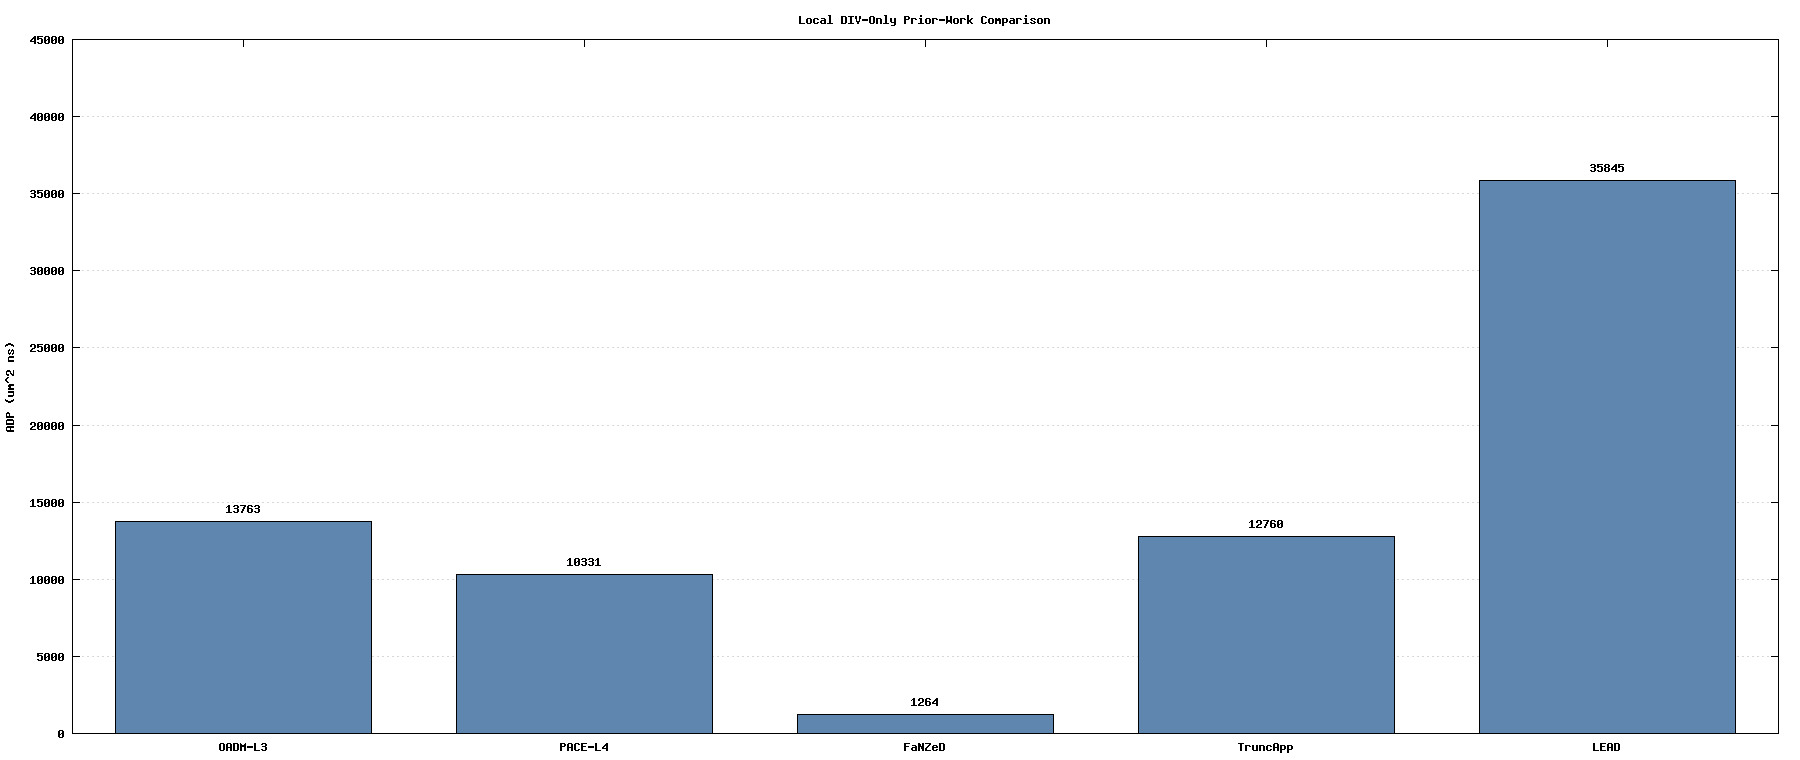
\includegraphics[width=0.94\textwidth]{pictures/priorwork_adp.png}
\caption{Area--delay product of the locally reproduced DIV-only designs under
the common explicitly flattened 10-ns DC/PT flow. QIAD is omitted from the
plot because its substantially larger ADP would compress the remaining bars;
its complete result remains reported in the accompanying result CSV.}
\label{fig:priorwork-adp}
\end{figure*}

Taken together, the measurements support two bounded claims. Against an
unshared exact selectable DIV+MUL reference, OADM substantially reduces area
and vectorless power. In DIV-only mode, it reaches competitive accuracy with
PACE but does not lead every PPA metric. Keeping these claims separate is
necessary because the two comparisons answer different architectural questions.

The remaining evaluation work follows directly from those boundaries. A
DIV/MUL-relevant workload is needed to connect L3 numerical error to application
quality. The present power figures are fair vectorless estimates rather than
workload-signoff energy, so a VCD/SAIF campaign is required for energy claims.
Placed-and-routed extracted PPA at common corners would strengthen the
fixed-level comparison. Exact-baseline claims remain limited to finite-normal
arithmetic until special values and subnormals are evaluated.

\section{Conclusion}
OADM realizes the OAD/OAM tangent-plane relation as one runtime-configurable
FP32 divider--multiplier with L0--L3 selection. Because the divider base and
level corrections are algebraically related to the multiplier plane, the design
shares partitioning, residual formation, plane evaluation, and the FP shell.
Under the common TSMC65 DC/PT flow, L3 reduces area, delay, and vectorless
power against an unshared exact DIV+MUL reference. Its DIV-only mode is
accuracy-competitive with PACE, although PACE remains the smaller DIV-only
implementation. OADM's contribution is thus a configurable unified arithmetic
block with measured structural sharing, not an assertion of best-in-class
performance for every DIV-only metric.

\begin{thebibliography}{18}
\bibitem{chen2020oam}
C. Chen, S. Yang, W. Qian, M. Imani, X. Yin, and C. Zhuo,
``Optimally approximated and unbiased floating-point multiplier with runtime
configurability,'' in \emph{Proc. IEEE/ACM ICCAD}, 2020, pp. 1--9.
\bibitem{oad2023}
P. Dong and C. Zhuo, ``OAD: Optimally approximated floating-point divider
with runtime configurability,'' working manuscript, 2023.
\bibitem{wen2025pace}
C. Wen, H. Du, J. Wang, Z. Chen, L. Zhang, Q. Sun, and C. Zhuo,
``PACE: A piece-wise approximate floating-point divider with runtime
configurability and high energy efficiency,'' \emph{ACM Trans. Des. Autom.
Electron. Syst.}, vol. 30, no. 2, Art. 21, 2025,
doi: 10.1145/3706634.
\bibitem{ebrahimi2020simdive}
Z. Ebrahimi, S. Ullah, and A. Kumar, ``SIMDive: Approximate SIMD soft
multiplier-divider for FPGAs with tunable accuracy,'' in \emph{Proc. GLSVLSI},
2020.
\bibitem{chen2015nonrestoring}
L. Chen, J. Han, W. Liu, and F. Lombardi, ``Design of approximate unsigned
integer non-restoring divider for inexact computing,'' in \emph{Proc. GLSVLSI},
2015, pp. 51--56, doi: 10.1145/2742060.2742063.
\bibitem{hashemi2016dynamic}
S. Hashemi, R. I. Bahar, and S. Reda, ``A low-power dynamic divider for
approximate applications,'' in \emph{Proc. DAC}, 2016, pp. 1--6,
doi: 10.1145/2897937.2897965.
\bibitem{imani2019cade}
M. Imani, R. Garcia, A. Huang, and T. Rosing, ``CADE: Configurable approximate
divider for energy efficiency,'' in \emph{Proc. DATE}, 2019, pp. 586--589,
doi: 10.23919/DATE.2019.8715112.
\bibitem{melchert2019saadi}
J. Melchert, S. Behroozi, J. Li, and Y. Kim, ``SAADI-EC: A quality-configurable
approximate divider for energy efficiency,'' \emph{IEEE Trans. VLSI Syst.},
vol. 27, no. 11, pp. 2680--2692, 2019,
doi: 10.1109/TVLSI.2019.2926083.
\bibitem{oelund2023ilafd}
J. Oelund and S. Kim, ``ILAFD: Accuracy-configurable floating-point divider
using an approximate reciprocal and an iterative logarithmic multiplier,'' in
\emph{Proc. GLSVLSI}, 2023, pp. 639--644,
doi: 10.1145/3583781.3590262.
\bibitem{saadat2019fanzed}
H. Saadat, H. Javaid, and S. Parameswaran, ``Approximate integer and
floating-point dividers with near-zero error bias,'' in \emph{Proc. DAC},
2019, doi: 10.1145/3316781.3317773.
\bibitem{vahdat2017truncapp}
S. Vahdat, M. Kamal, A. Afzali-Kusha, M. Pedram, and Z. Navabi,
``TruncApp: A truncation-based approximate divider for energy efficient DSP
applications,'' in \emph{Proc. DATE}, 2017,
doi: 10.23919/DATE.2017.7927254.
\bibitem{ratnaparkhi2022lead}
O. G. Ratnaparkhi and M. Rao, ``LEAD: Logarithmic exponent approximate divider
for image quantization application,'' in \emph{Proc. GLSVLSI}, 2022,
doi: 10.1145/3526241.3530323.
\bibitem{liu2023qiad}
H. Liu, M.-J. Wang, and M. Liu, ``QIAD: A quadratic interpolation approximate
divider,'' \emph{IEICE Electronics Express}, vol. 20, no. 11, 2023,
doi: 10.1587/elex.20.20230167.
\bibitem{wu2015curve}
L. Wu, ``A curve fitting approach for non-iterative divider design with
accuracy and performance trade-off,'' in \emph{Proc. NEWCAS}, 2015,
doi: 10.1109/NEWCAS.2015.7182097.
\bibitem{wu2024plsad}
L. Wu \emph{et al.}, ``Area-delay-energy-efficient approximate dividers
based on piecewise linear fitting of surface,'' 2024.
\bibitem{Ieee}
\emph{IEEE Standard for Floating-Point Arithmetic}, IEEE Standard 754-2008,
pp. 1--70, 2008.
\end{thebibliography}
\end{document}
